\chapter{Исследовательская часть}

\section{Технические характеристики}
Технические характеристики устройства, на котором выполнялись замеры по времени, представлены далее.

\begin{itemize}
	\item Процессор: AMD Ryzen 5 5500U\,--\,2.10 ГГц;
	\item Оперативная память: 16 ГБайт;
	\item Операционная система: Windows 10 Pro 64-разрядная система версии 22H2.
\end{itemize}

При замерах времени ноутбук был включен в сеть электропитания и был нагружен только системными приложениями.

\section{Демонстрация работы программы}
На рисунке \ref{img:demonstration} представлена демонстрация работы разработанного ПО, а именно показаны результаты работы алгоритмов поиска расстояний Левенштейна и Дамерау~---~Левенштейна на примере двух строк \textit{<<секста>>} и \textit{<<септима>>}.  
\clearpage
\begin{figure}[h]
	\centering
	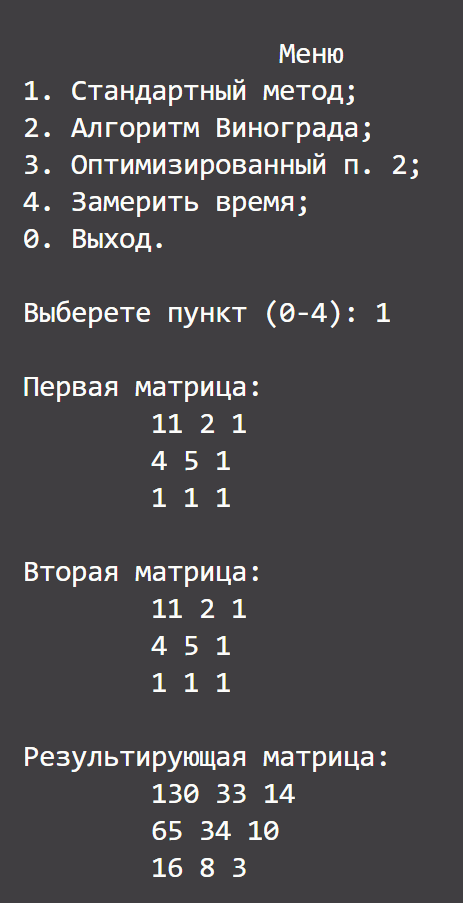
\includegraphics[height=0.7\textheight]{img/prog_work.png}
	\caption{Демонстрация работы программы}
	\label{img:demonstration}
\end{figure}

\clearpage

\section{Временные характеристики}

Результаты замеров приведены в таблицах \dots

На рисунках ... приведены графики зависимостей работы алгоритмов от размеров матриц.

Поскольку замеры по времени имеют некоторую погрешность, замеры производились 100 раз, а затем вычислялось среднее арифметическое значение.

% На рисунке \ref{plt:time_03} представлен график, иллюстрирующий зависимость времени работы от длины строк для итеративной реализации и рекурсивной реализации с использованием кеша алгоритма поиска расстояния Дамерау~---~Левенштейна. 
% \begin{figure}[H]
% 	\centering
% 	\includegraphics[height=0.5\textheight, page=3]{img/figures.pdf}
% 	\caption{Сравнение по времени итеративной реализации и рекурсивной реализации с использованием кеша алгоритма поиска расстояния Дамерау~---~Левенштейна}
% 	\label{plt:time_03}
% \end{figure}


\section*{Вывод}